\section{Tuning systems}

\bi

\i An International Conference in London
in 1939 established
A$_4$ = 440~Hz as the standard reference frequency.
Before that time, A$_4$ was tuned to different
frequencies ranging from 422.5~Hz (Handel) to
444~Hz, depending on composer, orchestra, ...

\i A tuning system is basically an assignment
of precise frequencies to all the other 
musical notes.

\i Since notes an octave apart have a frequency
ratio of exactly 2 in all tuning systems,
it suffices to assign frequencies to all the
notes within a single octave scale.  
The frequencies of notes outside this reference 
octave scale are simply related to the 
frequencies of the notes within the reference octave.

\i \ex
The note A$_3$ has frequency $440/2 =220~{\rm Hz}$
in all tuning systems.
 
\i In this section, we describe three different
tuning systems:
equal temperament, Pythagorean temperament, 
and just temperament.

\i As we shall see below, there is no such thing
as a perfect tuning system.
Each tuning system has its own advantages and 
disadvantages.

\ei
%%%%%%%%%%%%%%%%%%%%%%%%%%%%%%%%%%%%%%%%%%%
\subsection{Equal temperament}
\bi

\i Equal temperament is the most common 
tuning system in use today.

\i In equal temperament tuning, 
all semitone intervals have the same size, 
corresponding to a frequency ratio of 
%
\be
2^{1/12} = 1.05946
\ee
%
A {\em whole tone} is exactly equal to two semitones.

\i An equal-tempered chromatic scale was 
originally proposed independently 
by Vincenzo Galilei  (father of Galileo Galilei)
and Chu Tsai-Yu (a Chinese scholar) around 1580.

\i Equal temperament didn't become popular 
until the 1700's.
``The Well-Tempered Clavier" by Johannes Sebastian Bach 
demonstrated the usefulness of equal-temperament.
Using all 24 major and minor keys, this piece sounded
good only in equal-tempered tuning, and not in the other
tuning systems that we will describe below.

\i Table~\ref{t:equal-temperament} gives the frequency
ratios for a chromatic scale in equal-temperament tuning.
%
\begin{table}[htbp]
\begin{center}
\begin{tabular}{|c|c|}
\hline
Note & ET freq ratio \\
\hline
C & $2^{0/12}=1.000$ \\
C$^\sharp$/D$^\flat$ & $2^{1/12}=1.059$ \\
D & $2^{2/12}=1.122$ \\
D$^\sharp$/E$^\flat$ & $2^{3/12}=1.189$ \\
E & $2^{4/12}=1.260$ \\
F & $2^{5/12}=1.335$ \\
F$^\sharp$/G$^\flat$ & $2^{6/12}=1.414$ \\
G & $2^{7/12}=1.498$ \\
G$^\sharp$/A$^\flat$ & $2^{8/12}=1.587$ \\
A & $2^{9/12}=1.682$ \\
A$^\sharp$/B$^\flat$ & $2^{10/12}=1.782$ \\
B & $2^{11/12}=1.888$ \\
C$'$ & $2^{12/12}=2.000$ \\
\hline
\end{tabular}
\caption{Notes in a chromatic scale and the 
corresponding equal-temperament frequency ratios.}
\label{t:equal-temperament}
\end{center}
\end{table}

\i On a piano, or any instrument tuned to
equal temperament, the sharps and flats are equal
to one another---e.g., C${}^\sharp$ and D${}^\flat$
are tuned to the same frequency.
These are called {\em enharmonic} notes.

\i NOTE!! This equality of sharps and flats is
{\em not} true, in general, for other tuning systems
such as Pythagorean or just temperament 
(see below).
For these systems, one must first decide to tune,
for example, to either C$^\sharp$ or D$^\flat$, etc.

\i It is common to choose:
% 
\be
{\rm C}-{\rm C}^\sharp-{\rm D}-{\rm E}^\flat-{\rm E}-%
{\rm F}-{\rm F}^\sharp-{\rm G}-{\rm A}^\flat-{\rm A}-%
{\rm B}^\flat-{\rm B}-{\rm C}'
\nonumber
\ee
%
as the fundamental notes in a chromatic scale.

\i \exer 
Show that middle C in equal temperament has a frequency
of $261.63~{\rm Hz}$:
%
\be
{\rm C}_4:\quad 
{\rm A}_3 \cdot 2^{3/12} =
\frac{440\ {\rm Hz}}{2}\cdot 2^{3/12} = 261.63~{\rm Hz}
\ee

\ei
%%%%%%%%%%%%%%%%%%%%%%%%%%%%%%%%%%%%%%%%%%%
\subsection{Pythagorean temperament}
\bi

\i Pythagorean temperament is a tuning system 
constructed from just fifths and the the octave
(or, equivalently, from just fifths and fourths).

\i Using the circle of fifths (cf.~Fig.~\ref{f:circle-of-fifths}),
we can tune
a chromatic scale to Pythagorean
temperament as illustrated in Figure~\ref{f:pythagorean-chromatic-scale}.
%
\begin{figure}[htbp]
\begin{center}
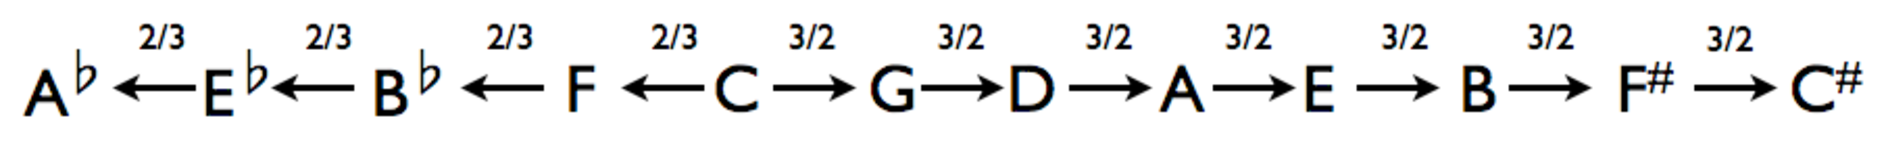
\includegraphics[width=\textwidth]{pythagorean-chromatic-scale}
\caption{A portion of the circle of fifths 
for calculating a chromatic scale of frequencies in Pythagorean temperament.}
\label{f:pythagorean-chromatic-scale}
\end{center}
\end{figure}
%

\i Applying the appropriate number of factors of $3/2$ 
(or $2/3$) and then scaling by $1/2$ (or $2$) 
to bring the resulting frequency to within an octave
of C, we obtain the numbers
in Table~\ref{t:pythagorean-chromatic}.
%
%\begin{table}[htbp]
%\begin{center}
%\begin{tabular}{|c|c|}
%\hline
%Note & Freq ratio \\
%\hline
%C & 1:1 \\
%D & 9:8 \\
%E & 81:64 \\
%F & 4:3 \\
%G & 3:2 \\
%A & 27:16 \\
%B & 243:128 \\
%C$'$ & 2:1 \\
%\hline
%\end{tabular}
%\caption{Pythagorean diatonic scale.
%The Pythagorean diatonic whole-tone interval is 9:8 
%and the diatonic semitone interval is 256:243.}
%\label{t:pythagorean-diatonic}
%\end{center}
%\end{table}
%
%
\begin{table}[htbp]
\begin{center}
\begin{tabular}{|c|c|c|c|}
\hline
Note & Pyth freq ratio & ET freq ratio & Difference (cents) \\
\hline
C & $1:1=1.000$ & 1.000 & 0 \\
C$^\sharp$ & $2187:2048= 1.068$ & 1.059 & $14$ \\
D & $9:8=1.125$ & 1.122 & $4$ \\
E$^\flat$ & $32:27=1.185$ & 1.189 & $-6$ \\
E & $81:64=1.266$ & 1.260 & 8 \\
F & $4:3=1.333$ & 1.335 & $-2$ \\
F$^\sharp$ & $729:512=1.424$ & 1.414 & 12 \\
G & $3:2=1.500$ & 1.498 & 2 \\
A$^\flat$ & $128:81=1.580$ & 1.587 & $-8$ \\
A & $27:16=1.688$ & 1.682 & 6 \\
B$^\flat$ & $16:9=1.778$ & 1.782 & $-4$ \\
B & $243:128=1.898$ & 1.888 & 10 \\
C$'$ & $2:1=2.000$ & 2.000 & 0 \\
\hline
\end{tabular}
\caption{Pythagorean chromatic scale and comparison
to equal-tempered frequency ratios.
The Pythagorean diatonic whole-tone interval is 9:8.
The Pythagorean chromatic semitone interval is
either 256:243 or 2187:2048.}
\label{t:pythagorean-chromatic}
\end{center}
\end{table}

\i Table~\ref{t:pyth_vs_ET} compares Pythagorean and
equal-tempered frequencies for all notes on the 
circle of fifths traversed once in the clockwise direction
and once in the counter-clockwise direction.
%
\begin{table}[htbp]
\begin{center}
\begin{tabular}{|c|c|c|c|}
\hline
Note & Pyth freq ratio & ET freq ratio & Difference (cents) \\
\hline
D$^{\flat\flat}$ & 0.987 & 1.000 & $-23$ \\
C & 1.000 & 1.000 & 0 \\
D$^\flat$ & 1.053 & 1.059 & $-10$ \\
C$^\sharp$ & 1.068 & 1.059 & 14 \\
E$^{\flat\flat}$ & 1.110 & 1.122 & $-20$ \\
D & 1.125 & 1.122 & 4 \\
E$^\flat$ & 1.185 & 1.189 & $-6$ \\
D$^\sharp$ & 1.201 & 1.189 & 18 \\
F$^\flat$ & 1.249 & 1.260 & $-16$ \\
E & 1.266 & 1.260 & 8 \\
F & 1.333 & 1.335 & $-2$ \\
E$^\sharp$ & 1.352 & 1.335 & 22 \\
G$^\flat$ & 1.405 & 1.414 & $-12$ \\
F$^\sharp$ & 1.424 & 1.414 & 12 \\
A$^{\flat\flat}$ & 1.480 & 1.498 & $-22$ \\
G & 1.500 & 1.498 & 2 \\
A$^\flat$ & 1.580 & 1.587 & $-8$ \\
G$^\sharp$ & 1.602 & 1.587 & 16 \\
B$^{\flat\flat}$ & 1.665 & 1.682 & $-18$ \\
A & 1.688 & 1.682 & 6 \\
B$^\flat$ & 1.778 & 1.782 & $-4$ \\
A$^\sharp$ & 1.802 & 1.782 & 20 \\
C$^\flat$ & 1.873 & 1.888 & $-14$ \\
B & 1.898 & 1.888 & 10 \\
C$'$ & 2.000 & 2.000 & 0 \\
B$^\sharp$ & 2.027 & 2.000 & 23 \\
\hline
\end{tabular}
\caption{A comparison of notes in the Pythagorean 
and equal-temperament tuning systems going once around
the circle of fifths in both the clockwise and 
counter-clockwise directions.}
\label{t:pyth_vs_ET}
\end{center}
\end{table}

\i Note that the circle of fifths doesn't close since
B$^\sharp$ and C$'$ are not equal to one another.
In addition, C$^\sharp$ doesn't equal D$^\flat$,
C$^\flat$ doesn't equal B, B$^{\flat\flat}$ doesn't equal A,
etc.

\i Pythagorean comma: ratio of frequencies for B$^\sharp$
and C$'$:
%
\begin{equation}
\frac{{\rm B}^\sharp}{{\rm C}'}
= \frac{(3/2)^{12} (1/2)^6}{2/1} 
= \frac{(3/2)^{12}}{2^7}
= \frac{531441}{524288} 
= 1.0136
\end{equation}
%

\i The above is equivalent to the statement that 
12 fifths doesn't exactly equal 7 octaves.
They differ by a ratio of 1.0136, which corresponds to
an interval of 23 cents.

\i Pythagorean temperament (by construction)
has perfect fourths and fifths in the key of C, 
but in the key of C$^\sharp$, the
fifth from C$^\sharp$ to A$^\flat$ 
is too flat by a factor of the Pythagorean comma:
%
\be
\frac{{\rm A}^\flat / {\rm C}^\sharp}{3/2}=
\frac{(128/81)/(2187/2048)}{3/2}
= \frac{1}{1.0136}
\ee
%
This is called a {\em wolf fifth} due to its `howling' sound
(which I can't hear!).

\i \demo
Use the matlab routine playinterval.m to compare the 
fifths C to G and C$^\sharp$ to A$^\flat$ in 
Pythagorean temperament.

\i In addition, a Pythagorean third (e.g., from C to E)
differs signicantly 
from a just major third that has a frequency ratio of 5/4.
This difference is called the {\em syntonic comma}:
%
\begin{equation}
\delta
=\frac{81/64}{5/4} 
=\frac{81}{80}
= 1.0125
\end{equation}
%
Thus, a Pythagorean third is too sharp by just over 
1\% or approximately 22 cents.

\ei

%%%%%%%%%%%%%%%%%%%%%%%%%%%%%%%%%%%%%%%%%%
\subsection{Just temperament}
\bi

\i Just temperament is a tuning system constructed 
from perfect fifths, major thirds, and the octave 
(or, equivalently, from perfect fifths, perfect fourths,
major thirds, and minor sixths).
In the key of C-major, it has three beatless 
major chords and two beatless minor chords.

\i Using Figure~\ref{f:just-chromatic-scale} as a schematic
for going up and down in frequency by perfect fifths and 
major thirds, we obtain the frequency ratios given in
Table~\ref{t:just-chromatic}.
%
\begin{figure}[htbp]
\begin{center}
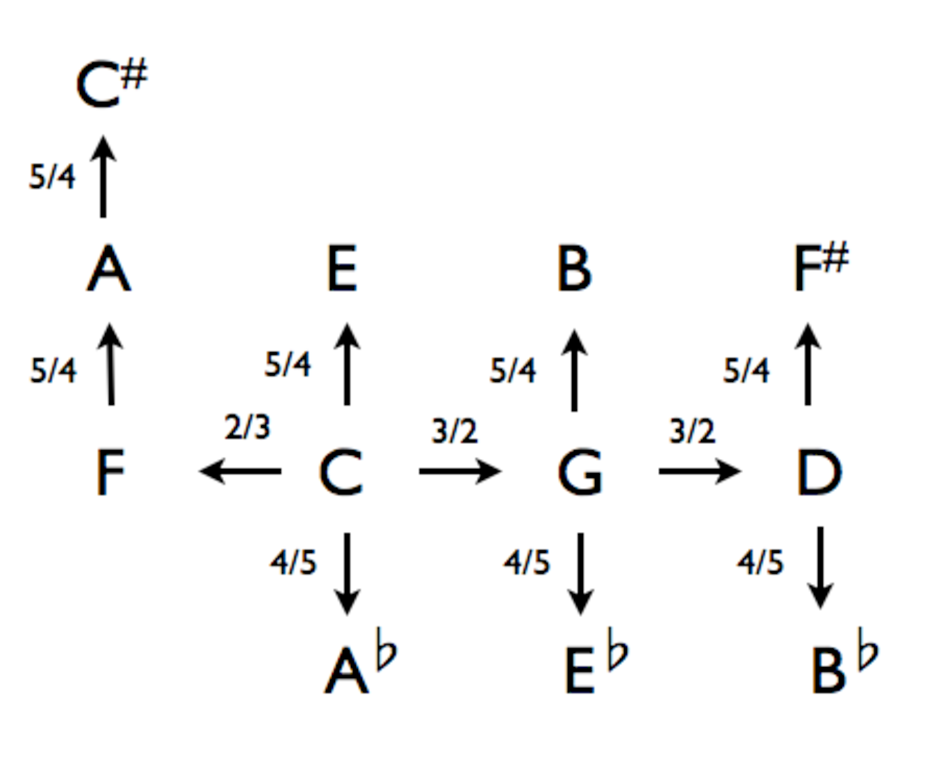
\includegraphics[width=.6\textwidth]{just-chromatic-scale}
\caption{Schematic for calculating a chromatic scale of frequencies 
in just temperament.}
\label{f:just-chromatic-scale}
\end{center}
\end{figure}
%
%\begin{table}[htbp]
%\begin{center}
%\begin{tabular}{|c|c|}
%\hline
%Note & Freq ratio \\
%\hline
%C & 1:1 \\
%D & 9:8 \\
%E & 5:4 \\
%F & 4:3 \\
%G & 3:2 \\
%A & 5:3 \\
%B & 15:8 \\
%C$'$ & 2:1 \\
%\hline
%\end{tabular}
%\caption{Just diatonic scale.
%The just diatonic whole-tone interval is either 9:8 or 10:9
%and the diatonic semitone interval is 16:15.}
%\label{t:just-diatonic}
%\end{center}
%\end{table}
%
\begin{table}[htbp]
\begin{center}
\begin{tabular}{|c|c|c|c|}
\hline
Note & Just freq ratio & ET freq ratio & Difference (cents) \\
\hline
C & $1:1 = 1.000$ & 1.000 & 0 \\
C$^\sharp$ & $25:24 = 1.042$ & 1.059 & $-29$ \\
D & $9:8=1.125$ & 1.122 & 4 \\
E$^\flat$ & $6:5=1.200$ & 1.189 & 16 \\
E & $5:4=1.250$ & 1.260 & $-14$ \\
F & $4:3=1.333$ & 1.335 & $-2$ \\
F$^\sharp$ & $45:32=1.406$ & 1.414 & $-10$ \\
G & $3:2=1.500$ & 1.498 & 2 \\
A$^\flat$ & $8:5=1.600$ & 1.587 & 14 \\
A & $5:3=1.667$ & 1.682 & $-16$ \\
B$^\flat$ & $9:5=1.800$ & 1.782 & 18 \\
B & $15:8=1.875$ & 1.888 & $-12$ \\
C$'$ & $2:1=2.000$ & 2.000 & 0 \\
\hline
\end{tabular}
\caption{Just chromatic scale and comparison to 
equal-tempered frequency ratios.
The just diatonic whole-tone interval is 
either 9:8 or 10:9.
The just chromatic semitone interval is 
either 16:15, 25:24, or 27:25.}
\label{t:just-chromatic}
\end{center}
\end{table}

\i Just temperament is arguably the best possible tuning 
system, provided one stays within the key in which 
you tuned to, e.g., the key of C for the above tuning.

\i But just as we saw for Pythagorean 
temperament, just temperament becomes increasingly out 
of tune as one move away from the key of C.
For example, the fifth C$^\sharp$ to A$^\flat$ in the
key of C$^\sharp$ differs from a perfect fifth by 41~cents.

\ei
%%%%%%%%%%%%%%%%%%%%%%%%%%%%%%%%%%%%%%%%%%%%%%
\subsection{Comparison of different tuning systems}
\bi

\i Figure~\ref{f:comparetemperaments} compares
the frequency ratios for a chromatic scale for
the three different tuning systems that we considered
in the previous subsections. 
One can easily see from this figure
that the fifth C$^\sharp$ to A$^\flat$ is too flat in
Pythagorean tuning and too sharp in just temperament
tuning.
%
\begin{figure}[htbp]
\begin{center}
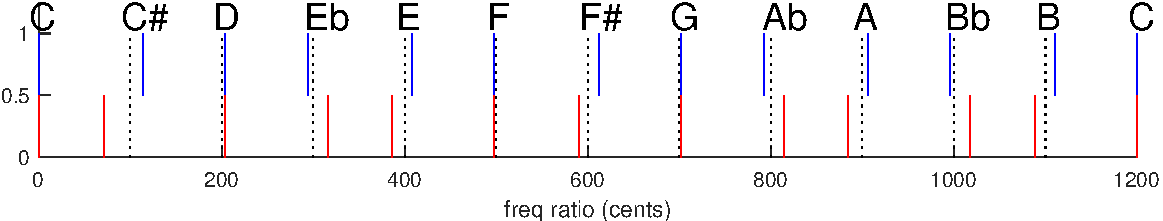
\includegraphics[width=.8\textwidth]{comparetemperaments.pdf}
\caption{Frequency ratios for a chromatic scale for 
the three different tuning systems that we considered.
The horizontal axis is the frequency ratio expressed in
cents (1200 cents equals one octave).
The dotted vertical lines correspond to equal-tempered
tuning (equally spaced at 0, 100, 200, $\cdots$ 1200~cents);
the blue and red vertical lines correspond to 
the Pythagorean and just temperament tuning systems, respectively.}
\label{f:comparetemperaments}
\end{center}
\end{figure}

\i Table~\ref{t:fifths} quantifies this comparison, 
giving the frequency ratios of two different fifths
(C to G and C$^\sharp$ to A$^\flat$) in the three different
tuning systems that we considered.
The last column gives the difference in cents between 
these frequency ratios and 3/2 for a just perfect fifth.
%
\begin{table}[htbp]
\begin{center}
\begin{tabular}{|c|c|c|c|}
\hline
Fifth & Temperament & Freq ratio & Difference (cents) \\
\hline
C-G & equal & 1.498 & $-2$ \\
C-G & pyth & 1.500 & $0$ \\
C-G & just & 1.500 & $0$ \\
C$^\sharp$-A$^\flat$ & equal & 1.498 & $-2$ \\
C$^\sharp$-A$^\flat$ & pyth & 1.480 & $-23$ \\
C$^\sharp$-A$^\flat$ & just & 1.536 & $41$ \\
\hline
\end{tabular}
\caption{Frequency ratios for two different fifths
for the three different tuning systems that we considered.
The last column is the difference in cents from
a perfect fifth, which has a frequency ratio of 3/2.}
\label{t:fifths}
\end{center}
\end{table}

\i \demo
Use the matlab routine fifths.m to compare the two
different fifths, C to G and C$^\sharp$ to A$^\flat$,
in the three different tuning systems that we considered.

\i There is no perfect tuning system.
Each system makes some compromise:

i) Equal temperament: Music in equal temperament 
can be played equally-well in all keys at the expense of 
imperfect intervals in all keys---e.g., a 
fifth doesn't have a frequency
ratio of 3/2, a major third doesn't have a frequency
ratio of 5/4, etc.
The circle of fifths closes.

ii) Pythagorean tuning has perfect fifths
in the key of C, but major thirds that 
are sharper than just major thirds by the 
syntonic comma $\delta = 1.0125$ (22 cents)
even in the key of C.
This means that major chords like 
C-E-G sound out of tune.
Also, even fifths are no longer perfect 
fifths when one moves away from the 
key of C---e.g., the wolf fifth 
C$^\sharp$ to A$^\flat$ is 23 cents too flat.

iii) Just temperament is the ideal tuning system
in the key of C having perfect fifths and major
thirds with frequency ratios of 3/2 and 5/4, 
respectively.
But just like Pythagorean tuning,
just temperament gets progressively worse as one 
moves away from the key of C---e.g., the 
fifth C$^\sharp$ to A$^\flat$ is now 41 cents too sharp.

\ei

